%%
%% DOCUMENT TYPE
%%

% general options:
% - inputenc        file encoding (should be "utf8" in most cases)
% - de/en           language of your work (influence pre-defined tokens)
% - declaration     adds the mandatory statutory declaration for theses
% - abstract        adds the abstract (from file "prelude_abstract.tex")
% - acknowledgment  adds an acknowledgment (from file "prelude_acknowledgment.tex")
%                   it is a nice gesture to personally thank people who
%                   supported you during your work.
% - symbollist      adds a list of symbols (from file "prelude_symbols.tex")
% - figurelist      adds and automatically creates a list of figures 
% - tablelist       adds and automatically creates a list of tables
% - index           generates an index based on the package "makeidx", please
%                   refer to its documentation for usage on index markup
% - bibbacklinks    adds backlinks from bibliography to the pages, where the
%                   corresponding entry is used (cited)
% - gray            make a gray-style version of the thesis report
%
% PhD thesis specific options
% - cv              adds your cv
% - publishsize     changes the page size from A4 to A5 for print publishing
%                   (please change the font size to 9pt, if you use this option)
% - approved        use this option, after your thesis has been formally approved
%                   (this will change the front page to meet formal/legal requirements)
% - ownpub          adds a second bibliography (from file "ownpub.bib") for your own
%                   publications related to the PhD thesis. According to the latest
%                   examination regulations, own work should be part of the regular
%                   bibliography (this option is hence obsolete)

\documentclass[en,abstract,acknowledgment,symbollist,inputenc=utf8]{tuhhthesis}


%%
%% SETUP BLOCK
%%

% thesis type, must be one of the following
% - projectwork
% - bachelorthesis
% - masterthesis
% - diplomathesis
% - phdthesis
\setthesistype{masterthesis}

% your full name as printed on any official document (e.g., passport)
\author{Christian Renner}

% the official title of your work (*must* match the filed title)
\title{A Brief Guide for Using the Telematics Thesis Class}

% the institution of the first examiner (refer to tuhhlangnames.def)
\institute{InstTelematics}

% date of submission as DD.MM.YYYY
\submitdate{04.05.2017}

% your matriculation number (for anything but PhD thesis)
\matrnumber{1234567890}

% PhD thesis only
%\setSexOfAuthor{male}
%\setBirthplace{Winsen/Luhe, Deutschland}
%\setPhDType{ing}

% your course of studies
\course{Informatik-Ingenieurwesen}

% full name and affiliation of first and second examiner
\examinerFirst{Prof. Dr. Volker Turau}{Institute of Telematics\newline Hamburg University of Technology}
\examinerSecond{Prof. Dr.-Ing. Bernd-Christian Renner}{Research Group smartPORT\newline Hamburg University of Technology}

\supervisorFirst{Christoph Weyer}{Institute of Telematics, Hamburg University of Technology}
%\supervisorSecond{Volker Turau}{Institute of Telematics, Hamburg University of Technology}

% optional: print the TUB document number on title page
% this only applies, if the document is formally publish under
% a TUB document number
%\tubdoknumber{4711}


% Curriculum Vitae
% only needed for thesis type PhD
%\usepackage[]{currvita}
%\setlength{\cvlabelwidth}{50mm}
%\renewcommand*{\cvlistheadingfont}{\normalfont\sffamily\large\color{tuhh_blue}}
%\renewcommand*{\cvlabelfont}{\normalfont\rmfamily\normalsize\color{tuhh_darkgray}}



%%
%% CONTENT AREA
%%

% mathematical symbols
% absolute value, ceiling, floor
\newcommand{\abs}[1]{\left|{#1}\right|}
\newcommand{\floor}[1]{\left\lfloor{#1}\right\rfloor}
\newcommand{\ceil}[1]{\left\lceil{#1}\right\rceil}

% regular sets %
\newcommand{\setN}{{\mathbb N}}
\newcommand{\setZ}{{\mathbb Z}}
\newcommand{\setQ}{{\mathbb Q}}
\newcommand{\setR}{{\mathbb R}}
\newcommand{\setC}{{\mathbb C}}
\newcommand{\classNP}{{\cal {NP}}}
\newcommand{\classP}{{\cal {P}}}

% a node and a sink
\newcommand{\node}{v}
\newcommand{\sink}{\node_{0}}          % sink

% Node Related Sets
\newcommand{\Network}{G}
\newcommand{\setNodes}{{\mathcal V}}% set of nodes
\newcommand{\setLinks}{{\mathcal E}}% set of edges
\newcommand{\setNeighbors}[1]{{\mathcal N}_{#1}}% neighbors
\newcommand{\setTree}{{\mathcal T}}% tree
\newcommand{\setChildren}{{\mathcal C}}%
\newcommand{\setLeafs}{{\mathcal F}}%
\newcommand{\numNodes}{N}%
\newcommand{\numChildren}{C}%

% density
\newcommand{\nodeDensity}{\varrho}

%% EOF



\begin{document}

% The Chapters
\chapter{Introduction}
%% Proposed roadmap
%
%   The use of RT in the industrial environments
%   Current standards IEEE and IEC and the TSN
%           Roadmap of standards
%           RTE protocols and OPC UA   
%           How are they related
%  
%   -----------State of the art--------------------------------
%   Applications with RTE and OPC UA in Hard Real Time applications     
%   A brief overview about the RT tools in robotics
%           The importance of EtherCAT as an open RTE protocol within robotics
%   Comparison of openess
%   EtherCAT introduction (selected by Hans Robot)
%           Focus on EtherCAT XoE <<THIS ONLY NEEDS TO BE MENTIONED
%------------------Out of scope--------------------------------------
%   HW ASICS and stuff like that
%   SW Stacks for EtherCAT development and other RTEs
%
%

% Terms:
% ACB = Axis communication board, alias for embedded communication hub for sensor data acquisition in a robotic system
% RTE = Real-Time Ethernet as specified in IEC 61784-2:2019. \cite{rte:standards}
% IIoT = Industrial Internet of Things

% 100/100
This document describes the different stages through the development of an embedded communication hub for sensor
data acquisition in a robotic system, that will be the starting point of a framework for the development of 
devices used within an industrial robot. In this document the prototype will be referred as \emph{Axis Communication Hub} or ACB. 

During this first chapter a brief introduction to the Real-Time Ethernet (RTE) industrial networks is presented, as well as 
a summary of the standards involved with comments about how they are related to each other. 
The second chapter shows a summary of the state of the art regarding the possibilities for developing open source projects 
according to the degree of openness of an RTE communication protocol. Moreover, the usage of these RTE 
industrial protocols in embedded applications and its relation to the Industrial Internet of Things (IIoT) necessities is 
briefly introduced. At the end of this chapter, a brief comparison of the openness of these protocols and how this is related 
to the development of devices is presented.  The applications introduced have to do mainly with EtherCAT, as it is within 
the scope of this Research Project, showing advantages that will be detailed as the reader reads through this document. 
Afterwards, the third chapter deals with the technical specification of this Research Project and its development proposal, 
including the hardware available, firmware structure and the overall prioritization of the goals. 
Later on, during the fourth chapter, the main points related to the implementation process are presented. 
In chapter five the overall results are discussed, where the reader can find comments about the implementation and test 
challenges and their solutions. In the sixth chapter the conclusions are summarized. 
Finally, extra information focused on the technical details of the project, such as diagrams or protocol-related specifications, 
can be found within the appendixes.

\section{The need of RT within industrial environments}

During the last years an increase in the usage of the Ethernet-based field buses within industry has been recorded. This
shows the expected adaptation of the industrial automation to the IT infrastructure, which is fundamental for the \emph{Industry 4.0} paradigm
and its consequent huge amount of data to be monitored, analyzed and controlled. This data deals at the same time with different time constraints 
and interconnectivity among the different layers of an industrial system and all their devices. 
Having in mind that the former \emph{automation pyramid}, see in Fig.~\ref{fig:pyramid-classic}, where the different layers needed various gateways
to communicate in a rather vertical approach, has been evolving to a one more flexible structure; it is then understandable 
that several technologies providing this access have been meeting each other while coming either from the top or the down levels. A good 
overview of the mentioned structures can be read in \cite{tsn_intro}.
Nowadays, these technologies offer similar features regarding data access and security, each of them with their own development 
history, alliances and, therefore, standards. 
\begin{figure}[h]
    \centering
    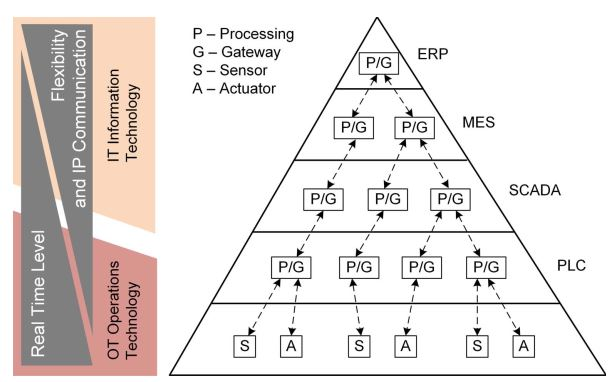
\includegraphics[width=0.7\textwidth]{imgs/intro-industryarchitecture2.jpg}
    \caption{Classical automation pyramid structure, source from \cite{tsn_intro}.}
    \label{fig:pyramid-classic}
\end{figure}

Coming from top-level-related frameworks, there is, e.g., the OPC UA project; whereas names like Profinet,
DeviceNET, EtherCAT, Powerlink, etc, come from the field bus side---the lowest level. All of them have developed in an individual way as response
to market needs, however meeting in the late decade through the necessity for unified standards to improve interoperability between the incredible number
of projects. This happens at a time were information, technical as well, and development tools have become even more available and
open to the end-user and the developer. Leading then now to a situation where the private initiatives are not any longer the full owners of the technology development.
See Fig.~\ref{fig:pyramid-iiot} for the IIoT's approach.

\begin{figure}[h]
    \centering
    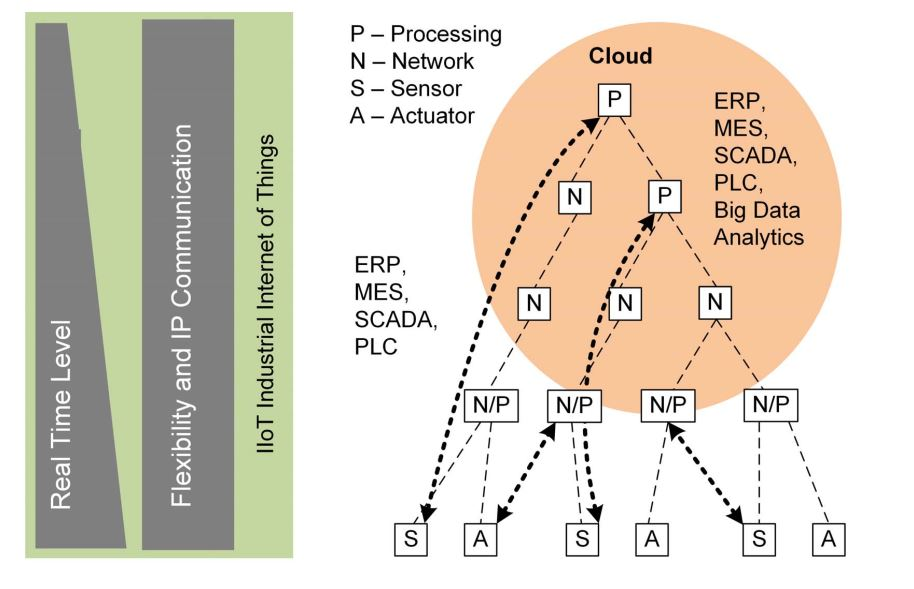
\includegraphics[width=0.7\textwidth]{imgs/intro-industryarchitecture.jpg}
    \caption{\emph{Industry 4.0} a more flexible automation structure. Industrial Internet of Things, source from \cite{tsn_intro}.}
    \label{fig:pyramid-iiot}
\end{figure}

Another line of work, closely related to interoperability, is the Real Time (RT) applications in their both versions with \emph{hard} and \emph{soft} requirements. 
Nowadays, there is an increasing number of applications in robotics that demand control loops and device chains that
require hard real time performance. Although these requirements are more common at the operational technology level, such as, robots, CNCs, servo motors, etc. 
They all face now the IIoT demands; hence, their networks should meet as well certain degree of RT capability. 
Moreover, synchronization of time sensitive
systems within manufacturing lines, for instance, has been addressed for years by the RTE protocols and now this kind of features are increasingly
been demanded as well at upper layers.

The current automation industry has many competitors and close technologies, as a natural consequence for specific processes requirements---depending on the industry;
but also as a response of the market. However, the search for standardization
can be tracked back to the 1980s, as the field buses were standardized by the International Electrotechnical Commission (IEC). 
This continued and Ethernet took its place within the industry. As an important note, during the last two years, according to the HMS Industrial Networks' annual study,
the total market shares of new industrial nodes in factory automation increased for the Industrial Ethernet from \num{52}$\%$ to \num{64}$\%$; while the
field buses decreased in the same period from $42\%$ to only $30\%$. Finally, the industrial wireless remained around the \num{6}$\%$, see Fig.\ref{fig:fieldbus_shares}.

It is yet worthy to mention that the name \emph{Industrial Ethernet} is used only as a 
generalization for the group of protocols that historically developed on IEEE's Ethernet specification; even though they all are almost no further
compatible with each other---because of the modified Media Access Control (MAC) layers. 
Details about the differences is addressed in the following chapters.  

\begin{figure}[h]
    \centering
    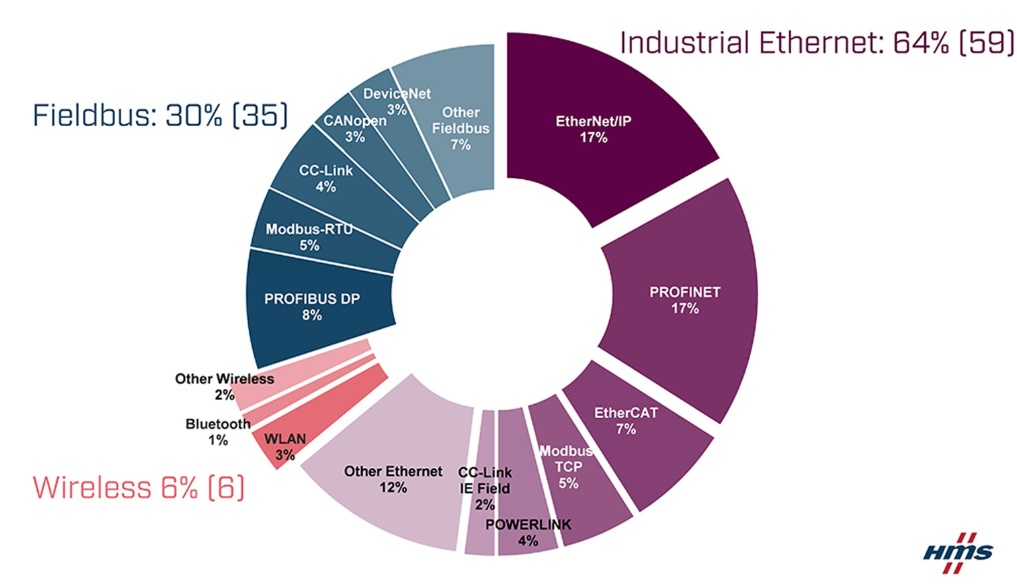
\includegraphics[width=.8\textwidth]{imgs/intro-buses-share.jpg}
    \caption{Industrial network market shares 2020 according to HMS Networks. Source from \cite{fieldbus_shares}.} %Add the reference, this could be a table
    \label{fig:fieldbus_shares}
\end{figure}

Vendor protected technology has its limit when there are plenty of possibilities for automation technologies, even if they are in ongoing development. 
For instance, as happened during the lifetime of the Open Platform Communications (OPC) project---predecessor of OPC UA---that was started only upon Microsoft Windows and 
as the time went by, the emerging needs made it change to use open standards and a multiplatform approach.

To introduce the reader to a common ground regarding standardization, the following section will present a brief summary of the standards that 
are of interest for anyone who wants to start developing using industrial interfaces.

\section{Industrial standards and the TSN initiative}\label{sec:standards} 

This section is intended to provide the starting developer a rough but useful reference of the standards related to industrial 
communication networks. 

First, due to the historical and technological process of innovation within the information and communication 
systems, several parties have been related and, at some extension have merged results, bringing out an interconnected 
set of norms that thrive continuously onto a global standardization.

The following list is intended to be a quick reference to the current standards for Ethernet, legacy and current field buses, 
Time-Sensitive Networks in their American and international initiatives. This way, the reader has a roadmap to be taken into
account for deeper research within the industrial applications. 
Furthermore, information related to the similar standardization processes between 
the IEC, ISO and IEEE, and their unavoidable cooperation, can be read in \cite{standards_coop}. %a comparisson of the ieee and iec standars processes

\begin{description}
    \item[ISO/IEC/IEEE 8802-3:2015] Revision of the Ethernet standard for half and full-duplex communication up to \SI{100}{\mega\bit\per\second}. 
    Originally published by American IEEE 802-3 in 1985 and accepted internationally in 1989. The last revision 8802-3-2017/Amd 10-2019 includes
        MAC controls for \SIlist{200;400}{\giga\bit\per\second}. More information in \cite{iso8802_ethernet}. %https://www.iso.org/standard/72048.html 
        After 2019 The name Ethernet is not longer used, instead CSMA/CD or a reference to the corresponding ISO standard 8802.3 is the formal name.
    \item[IEC 61158:1999-2000] First international field bus standard published in 1999, where 8 \emph{Types} of field buses were introduced addressing the 
        Physical Layer (PhL), the services and protocols of Data Link Layer (DLL) and Application Layer (AL). Some included brand 
        names were the following: H1/HSE/H2, ControlNet, EtherNET/IP, Profibus, Profinet, Interbus. This standard has an interesting story
        concluding with the signing of the \emph{Memorandum of Understanding} by the main contenders to put end to the field bus war. The latter can be reviewed in \cite{fieldbus_history}.%The Fieldbus Standards: History and Structures
         The standard's most updated version in 2019 includes 26 Types of protocols, creating out of them the so-called Communication Profiles (CP), likewise grouped
        into field bus Communication Profile Families (CPF). 
    \item[IEC 61784-Part 2:2008] It is extension for the RT capable CPs that are based on the IEEE 8802-3 standard. Commercial names included 
        are the next: EtherCAT, Profinet, Ethernet/IP, Ethernet Powerlink, and Modbus TCP. An interesting overview of the current development 
        of the industrial communication networks can be reviewed in \cite{future_iiot}. %Industrial Communication Systems and Their Future Challenges: Next-Generation Ethernet, IIoT, and 5G
        The SERCOS CPF is highlighted, since its third version is, altogether with the EtherCAT profile, the fastest one in the list; providing as well
        a more efficient use of the available bandwidth with an open source resources. It shows even advantages over CAN devices due
        to its original design intended for hard RT motion control; for more information review \cite{sercos_origin} and \cite{sercos_performance}. %https://www.designnews.com/sercos-picks-pace %https://www.sercos.org/technology/advantages-of-sercos/performance/. 
        This is a very interesting hard RT protocol whose applications might need further study out of the scope of this 
        Research Project.
    \item[IEEE 802.1A/B/C/D/Q] Time-Sensitive Networking standards is an initiative to improve the IEEE 802-3 in order to meet the industrial real time requirements, 
        which story can be tracked back to 2005, as the IEEE 802-3 group was merged with the IEEE 802.1 Audio Video Bridging Task Group and started to work for
        industrial environments. This a response to the vast alternatives of the RTE CPs. About 60 individual IEEE standards oriented to improve
        the ISO/OSI layer 2, including 13 focused on its security, are within the scope of the TSN project. A nice introduction to this standard's scope can be read from TSN 
        section in \cite{future_iiot}. %section about the TSN
        The mentioned project covers the lower layers of the communication system, whereas the upper ones, representation and transfer of data, is
        addressed by OPC UA. Moreover, it is important to mention that this is an ongoing project and still around $40\%$ of its standards are
        in draft or preparation phase. For further information regarding the current standard development, visit \cite{tsn_homepage}.
    \item[IEC/IEEE 60802] TSN Profile for Industrial Automation is the stand alone TSN base standard that will include the common advancements
        from IEC SC65C/WG18 and IEEE 802 work groups mentioned in the previous item. See \cite{tsn_profile} for the current development group's activities. %https://1.ieee802.org/tsn/iec-ieee-60802/
        This is an ongoing project started around 2017, still being in a draft phase. Since this will be the international standard, it would be 
        the equivalent to the effort once given during the creation of the IEC 61158 for the legacy field buses.
    \item[IEC 62541:2016-2020] Set of IEC standards for OPC UA. Individually, the IEC 62541-14:2020 defines the OPC Unified Architecture 
        (OPC UA) PubSub communication model. It defines an OPC UA publish/subscribe pattern which complements the client server pattern defined 
        by the Services in IEC 62541-4. IEC TR 62541-1 gives an overview of the two models and their distinct uses. For the concrete list of contents, review \cite{opcua_standard}. %https://webstore.iec.ch/publication/61108  
        An overview of this technology and how it is planned to complement the TSN can be reviewed in \cite{opc_tsn_application}. %Open Source OPC UA PubSub over TSN for Realtime Industrial Communication
\end{description}



% CANopen protocol is not capable of hard real time capabilities?


% >>Here comes information about SERCOS. The SERCOS interface started as a project for providing a Hard Real Time capable communication
% bus, it has been developed during the years, having nowadays three versions. The first ones operating over a serial bus and submitted
% to the IEC, which in 1995 released it as IEC 61491.[2] After the release of the original standard, original working group member companies 
% including ABB, AEG, AMK, Robert Bosch, Indramat, and Siemens founded the "Interest Group Sercos" to steward the standard. \ref{dummy} %https://en.wikipedia.org/wiki/SERCOS_interface#cite_note-3
% Even though the capabilities meet hard real time requirments, compared to other technologies, is rather limited. %https://en.wikipedia.org/wiki/SERCOS_interface#cite_note-3
% For the last version it has been capable to address up to 60 Motion Axes and makes use of the Ethernet standard, making it an alternative
% for the mentioned technology comming from BEckhoff. Together with EtherCAT, Sercos is the fastest 100Mps industrial Ethernet technology.
% One advantage so far of this protocol is its parallel development with the OPC UA, making it natively compatible with such networks* 
% and security layers.



\chapter{Structure}

This chapter is intended to give you an overview about structuring your work. Note that the following instructions must be understood as a guideline. Of course, the final structure of your thesis report depends on the actual nature of the topic. For instance, the structure of pure theoretical work differs from that of implementational ones. Before starting structuring your work, discuss the actual content, chapters and sections with your supervisor.

\section{...}

Ok, this piece of writing is incomplete ... and reserved for some future version of this guide ...
\chapter{The TUHH Telematics Thesis Class}

In order to free you from reading through all the classes and packages provided with our Thesis Template, we will summarize the main parts for you. The root document of your thesis is the file \file{thesis.tex}. It contains global setup and the inclusion of the different chapters, which are outsourced to individual files, i.e., each chapter is organized in a dedicated file.

\section{Setup}

Before starting your thesis report, adjust all the personal and thesis related data in the root document. We will briefly cover this matter.


\subsection{Options}\label{sub:options}

If you have at look at the very first line of the root document, you'll discover the loaded document class along with its options. The most important options are:
\begin{description}
  \item[de] German Version (cannot be combined with option \texttt{en})
  \item[en] English Version, default (cannot be combined with option \texttt{de})
  \item[gray] Use this option to make a gray-style version of the thesis report
  \item[print] Use this option for your print version, i.e, switched off hyperref colors (this makes only sense for electronic versions)
  \item[declaration] Use this option for inclusion of the declaration by candidate
  \item[abstract] This option enables the automatic inclusion of an abstract, which is expected in the file \file{prelude\_abstract.tex}
  \item[acknowledgment] This option enables the automatic inclusion of an acknowledgment, which is expected in the file \file{prelude\_acknowledgment.tex}
  \item[symbollist] If you have a bunch of mathematical symbols, use this option in order to automatically include a list of symbols. The latter has to be provided the file \file{prelude\_symbols.tex}
  \item[cv] Use this option to include your curriculum vitae at the end of the document. The latter has to be provided the file \file{postlude\_cv.tex}. This is required for PhD theses.
  \item[ownpub] Use this option to include a list of your own publications. The latter has to be provided the file \file{ownpub.bib}. This is required for PhD theses. Make sure to also run \texttt{bibtex ownpub}, otherwise your own publications will not show up.
\end{description}


\subsection{Thesis Type}

Depending on the actual type of thesis, you have to use the correct parameter for the command \cmd{\textbackslash{}setthesistype}: \emph{bachelorthesis}, \emph{projectwork}, \emph{masterthesis}, \emph{diplomathesis}, and \emph{phdthesis}.


\subsection{Author, Title, and Date}

Next, you must specify your name, your matriculation number and course of studies, along with the title of the thesis, and the date of submission with the corresponding commands \cmd{\textbackslash{}author}, \cmd{\textbackslash{}matrnumber} \cmd{\textbackslash{}course}, \cmd{\textbackslash{}title}, and \cmd{\textbackslash{}date}. The latter of these takes two arguments: the actual, complete date of submission and a short version for the title page with month and year only.

A PhD thesis also requires the following values: 
\cmd{\textbackslash{}submitdate}, \cmd{\textbackslash{}setBirthplace} and \cmd{\textbackslash{}setPhDType}. The latter must be one of the values \emph{ing}, \emph{nat}, or \emph{pol}.

\subsection{Institute, Supervisor, and Examiner}

You can set up one or two examiners for your thesis, depending on the examination regulations for your thesis. This is done via the commands
\cmd{\textbackslash{}examinerFirst} and \cmd{\textbackslash{}examinerSecond}. Each of these takes two parameters: the name of the examiner and his or her affiliation, i.e., the institute and university (the latter two should be separated by \cmd{\textbackslash{}newline}).
You may also provide up to two supervisors (tutors) of your thesis. This is done via the commands \cmd{\textbackslash{}supervisorFirst} and \cmd{\textbackslash{}supervisorSecond}. The command requires the same two parameters as the examiner commands. However, the affiliation should make up a single line, i.e., separate institute and university by commas.
Finally, you have to specify the institute explicitly using the command \cmd{\textbackslash{}institute}. Available parameters are defined in the file \file{tuhhlangnames.def}. Most likely, you will need \emph{InstTelematics}.


\section{Building Blocks}

Your report consists of a couple of building blocks, which we will discover and explain in this section.


\subsection{Mathematical Symbols}

At the moment, there is one major hint for you: If there are going to be any mathematical symbols in your report, define a command for each of them in the file \file{setup\_math.tex}. First of all, this makes your sourcecode---and equations in particular---more readable. Secondly, symbols can be replaced or altered quickly and elegantly.

After the table of contents and before the first chapter of your report, show a table of all (mathematical) symbols used in your report with a brief explanation. An example is found in this document. Inclusion of such a list is explained in Sect.~\ref{sub:options}.


\subsection{Chapters}

Each chapter of your thesis should reside in a dedicated file. These files are linked into the thesis report via the \cmd{\textbackslash{}input} command. We do not discuss this matter in detail, but refer to the source code of this guide.


\subsection{Bibliography}

Since you're using \LaTeX, it's most suitable to employ BibTeX for your bibliography. By default, the bibliography is expected in the file \file{thesis.bib}. The specified style is a sincere recommendation. Information on required fields for the most important types of bibliography entries is provided in Sect.~\ref{sec:bib}.


\subsection{Appendix}

The appendix is organized as are the chapters: in separate files. In general, there should rarely be any need for a vast appendix. We only require you to have one appendix chapter for an attached CD/DVD with all your material, source code and the final versions (PDF) of your report and talk. If there are a few things that are related to your work, but do not suit into the main part, then these may go to the appendix. However, ask your supervisor before creating an appendix.


\subsection{Graphics and Plots}

If possible, try to draw your graphics with TikZ and the plots with Gnuplot with the TikZ terminal. TikZ is flexible, neat, and capable of using just the same fonts and symbols as used in and throughout your report. In general, create individual PDFs for each plot or graphic and insert it into your report using \cmd{\textbackslash{}includegraphics}. Doing so will speed up the compilation process. Ask your supervisor in case of any questions.


\chapter{Figures, Tables, and more}

In this chapter, figures, tables, and listings as available in this template are being introduced.\cite{NS2Manual}


\section{Figures}\label{sec:figures}

Figures should be frequently used throughout your thesis report, as they are a powerful instrument. Not only that one picture every two to three pages lightens up the work, a picture can even say more than a thousand words. However, note that a lonely figure is truly worthless. Make sure that you reference your figures in the text and that you explain them appropriately.

In the following, a set of useful commands for including figures into your work is introduced. Note that figures will be automatically placed by \LaTeX. You can rearrange figures be simply changing their position in the source code; however, you should not mess around with the figure placement options.


\subsection{Default yet Fancy Figures}\label{sub:simpleFigures}

Figures may require different display properties, so that a variety of different display styles are available. The main type of figures are illustrations. For these, the \cmd{\textbackslash{}fig} command is available. It has three parameters, which are the path to the picture, the caption, and the label. Labels of figures should have the prefix \cmd{fig:}. An example is shown in Figure~\ref{fig:simpleFigure}. The figure must be transparent, as it will be placed within a gray frame with a tiny border.

\fig{images/app_setup}{Figure with gray background box and border spacing. In this example, you also see what happens in case of a long caption.}{fig:simpleFigure}

In general, figures are displayed with a small inner spacing to the surrounding frame. As this may not be desired in some cases, there exists a version without additional spacing, \cmd{\textbackslash{}fignospacing}.


\subsection{The Frameless Variant}\label{sub:framelessFigures}

If you want to display photographs or illustrations, the surrounding frame and the gray background may be disturbing. Here, the command \cmd{\textbackslash{}fignoframe} jumps in and helps you out. The parameters are the same as described in Sect.~\ref{sub:simpleFigures}. See Fig.~\ref{fig:fignoframe} for a sample display.

\fignoframe{images/harvester}{Figure without surrounding frame and without gray background}{fig:fignoframe}


\subsection{Subfigures}\label{sub:subfigures}

When you start writing your evaluation and intend to display plots, having one plot per figure box is not a very handsome solution. Usually, you want to display multiple plots per figure box. This can be easily achieved using subfigures. In order to employ the neat and fancy boxing around your figures, use the \cmd{\textbackslash{}subfigbox}. As its first parameter, it takes a series of subfigures---using the \cmd{\textbackslash{}subfigure} command. Multiple rows are created using the \cmd{\textbackslash\!\textbackslash{}} command, automatic horizontal alignment is achieved via a \cmd{\textbackslash{}hfill} between adjacent figures in the same row. A possible layout is shown in Fig.~\ref{fig:trees}.

\subfigbox{
  \subfigure[complete]{\label{subfig:treeComplete}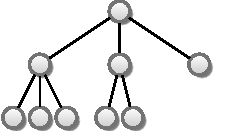
\includegraphics{images/tree_complete.pdf}}\hfill%
  \subfigure[min depth]{\label{subfig:treeMinDepth}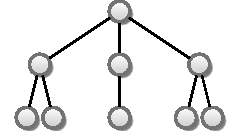
\includegraphics{images/tree_mindepth.pdf}}\hfill%
  \subfigure[full tree]{\label{subfig:treeFull}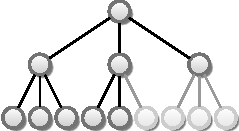
\includegraphics{images/tree_full.pdf}}%
}{Box with gray background intended to hold subfigures}{fig:trees}


%%
\section{Tables}\label{sec:tables}

Unfortunately, tables can be a pain in \LaTeX{} and have a clear tendency to look ugly. For this reason, we built the package \emph{tuhhtable}. A brief discussion of frequently used table pattern follow in dedicated subsections. 


\subsection{Simple Tables with Headings}\label{sub:simpleTables}

When creating tables, a couple of rules should be obeyed. Firstly, vertical lines are rarely helpful in tables. In contrast, they make a table harder to read in most cases, when people read from left to right. So try not to use them. To further support readability---while also hinting at eye candy---shaded rows are employed. To mark the end of a table and to separate the table body from the header, horizontal lines can be used. A recommended table layout is depicted in Table~\ref{tbl:simple}. Have a look at the source code of this document to understand how things work.\cite{MAC_Survey}

\begin{tuhhtable}
  \begin{tabular}[tp]{L{.3\textwidth}C{.3\textwidth}R{.3\textwidth}}
    \THc{1}{c}{Head 1} & \THc{1}{c}{Head 2} & \THc{1}{c}{Head 3} \\
    \THsub{1}{c}{sub 1} & \THsub{1}{c}{sub 2} & \THsub{1}{c}{sub 3} \\
    \abovebodyrule
    l1     & c1     & r1     \\\TRc
    l2     & c2     & r2     \\
    l3     & c3     & r3     \\\TRc
    \belowbodyrule
  \end{tabular}
  \caption{A simple table with a heading}
  \label{tbl:simple}
\end{tuhhtable}


\subsection{Special Table Elements}\label{sub:specialTableElements}

In case your are carrying out comparisons of, lets say, different algorithms, you might want to judge the quality of certain properties by symbols, such as '+', '-', or the like. Unfortunately, these symbols are not very fancy, so that we have defined a set of more eye-catchings ones. They are displayed in Table~\ref{tbl:elements}. Again, have a look at the source code of this document to understand how they can be used.

\begin{tuhhtable}
  \footnotesize\centering
  \begin{tabular}[tp]{L{.22\textwidth}C{.22\textwidth}C{.22\textwidth}C{.22\textwidth}}
    \THempty & \THc{1}{c}{Product 1} & \THc{1}{c}{Product 2} & \THc{1}{c}{Product 3} \\
    \abovebodyrule
    \TRh{1}{l}{has feature}  & \tblYes    & \tblYes  & \tblNo    \\\TRc
    \TRhc{1}{l}{usability}   & \tblGood   & \tblBest & \tblBad   \\
    \TRh{1}{l}{price}        & \tblNA     & \tblFair & \tblWorst \\\TRc
    \belowbodyrule
  \end{tabular}
  \caption{Special symbols for use in tables}
  \label{tbl:elements}
\end{tuhhtable}



\subsection{Advanced Tables}\label{sub:advancedTables}

Sometimes, a simple table layout as presented in the previous section is not sufficient. An example is shown in Table~\ref{tbl:advanced}. Hence, additional commands are available. 

% DECISION GUIDANCE TABLE
\begin{sidewaystable}
  \footnotesize\centering
  \begin{tabular}[htp]{lC{3.2cm}C{3.2cm}C{3.2cm}C{3.3cm}C{3.2cm}}
  \THempty    & \THc{1}{c}{Type I}   &
                 \THc{1}{c}{Type II}  &
                  \THc{1}{c}{Type III} &
                   \THc{1}{c}{Type IV}  &
                    \THc{1}{c}{Type V}  \\
%
  \TRx{6}{l}{Network Size}\\
  \abovebodyrule
  Small       & \tblWorst    & \tblGood     & \tblBest     & \tblBest     & \tblBad      \\\TRc
  Medium      & \tblFair     & \tblFair     & \tblGood     & \tblFair     & \tblFair     \\
  Large       & \tblBad      & \tblWorst    & \tblWorst    & \tblWorst    & \tblBest     \\
  \belowbodyrule
%
  \TRx{6}{l}{Density}\\
  \abovebodyrule
  Low         & \tblWorst    & \tblFair     & \tblBad      & \tblWorst    & \tblBad      \\\TRc
  Medium      & \tblFair     & \tblFair     & \tblFair     & \tblFair     & \tblGood     \\
  High        & \tblWorst    & \tblFair     & \tblGood     & \tblFair     & \tblGood     \\
  \belowbodyrule
%
  \TRx{6}{l}{Initial Fill Level}\\
  \abovebodyrule
  Low         & \tblFair     & \tblGood     & \tblBest     & \tblBest     & \tblGood     \\\TRc
  High        & \tblBad      & \tblBad      & \tblWorst    & \tblWorst    & \tblBest     \\
  \belowbodyrule
%
  \TRx{6}{l}{Variation of Initial Fill Levels}\\
  \abovebodyrule
  Low         & \tblBest     & \tblGood     & \tblBad      & \tblGood     & \tblBest     \\\TRc
  High        & \tblBest     & \tblBad      & \tblWorst    & \tblGood     & \tblBest     \\
  \belowbodyrule
%
  \TRx{6}{l}{Collisions and Packet Loss}\\
  \abovebodyrule
  Collisions / Yield &
    \tblYes / \tblWorst &
    \tblNo  / \tblBest &
    \tblNo  / \tblBest &
    \tblNo  / \tblBest &
    \tblYes / \tblFair     \\\TRc
  Packet Loss & \tblGood     & \tblFair     & \tblWorst    & \tblWorst    & \tblGood     \\
  \belowbodyrule
  \end{tabular}
  \caption{Characteristics of the TDMA schedules: Decision Guidance \cite{Renner:2008:Diploma}}
  \label{tbl:advanced}
\end{sidewaystable}



\section{Enumerations \& Co.}\label{sec:enumerations}

Feel free to use enumerations, itemizations, and the like to suit your needs. We have adjusted the itemization to match our slides class plus our color scheme. We thus discourage you from changing items or colors.



\section{Listings}\label{sec:listings}

For placing and typesetting listings, we encourage the use of the \emph{listings} package available for \LaTeX. Please have a look into the corresponding package manual. The facilitate the usage of this package, we have already set it up to follow the same look as the rest of our visual stuff. This includes the gray background, the frame, and appropriate colors. The package is automatically loaded by the template class and defines \emph{C++} as the default programming language---you are completely free to adjust the language, of course. A sample listing is displayed in Lst.~\ref{lst:sampleListing}. Note that all listings should have labels with the prefix \cmd{lst:} and should be referenced in the text. Besides complete listings, we have defined the command \cmd{\textbackslash{}cmd}, which display its first parameter text in monospace font.

\begin{lstlisting}[label=lst:sampleListing,caption={A simple C++ program for reading in positions}]
#include <iostream>                                                                       
#include <vector>                                                                         
#include <inttypes.h>                                                                     

using namespace std;

/* 2-D positions */
typedef struct pos_s {
        int16_t  x, y;
} pos_t;

int main(void)
{
        uint16_t       numData;
        vector<pos_t>  v;
        pos_t          tmp;

        /* read numData 2-D points */
        cin >> numData;
        for (unsigned i = 0; i < numData; i++) {
                cin >> tmp.x >> tmp.y;
                v.push_back(tmp);
        }
        cout << "read " << numData << " points" << endl;

        /* process data */
        process(v);

        return 0;
}
\end{lstlisting}

\chapter{Style Guide}\label{cha:styleGuide}

Finally, we want to give some advices and recommendations on styling. This does not relate to writing skills, which is gracefully embraced by the \emph{Chicago Writer's Manual}.


\section{Fonts}\label{sec:fonts}

Font setup etc. has been done for you by means of this very template. We hence expect you to follow the given style; meaning that we discourage you from changing font sizes, faces, families, colors, as well as line and paragraph spacing or any spacing in general.


\section{Citing and Referencing}\label{sec:citeAndRef}

Citing other sources and referencing parts of your work is quite easy using the commands \cmd{\textbackslash{}cite} and \cmd{\textbackslash{}ref}. Yet, let us mention some aspects. Firstly, when citing, you should make clear, somehow, which part is from the cited work and which is not. Secondly, you most likely want to place a tilde ($\sim$) between the word just in front of the \cmd{\textbackslash{}cite} or \cmd{\textbackslash{}ref} commands to avoid ugly looking line breaks. Thirdly, note that citations and references are proper parts of a sentence: Do not simply put them at the end of a sentence; use them as nouns!

More importantly, obey the following rules. Always capitalize when referencing, e.g., say Fig.~17 instead of fig.~17. You can abbreviate Figure with Fig., Section with Sect., and Listing with Lst. When referencing equations, simply place the number in parentheses---e.g., say (3.2) instead of Eq.~3.2---that's all. While you can certainly do this by hand, we encourage you to use the \emph{cleveref} package, which already does this for you. By using \cmd{\textbackslash{}cref} or \cmd{\textbackslash{}Cref} (at the beginning of a sentence) as a replacement for \cmd{\textbackslash{}ref}, the type of reference is automatically added. Please check the manual of the package for further details.

For your own sake, use a pattern for labels. We recommend to use prefixes for each type of label: chapters (\cmd{cha:}), sections (\cmd{sec:}), subsections and below (\cmd{sub:}), figures (\cmd{fig:}), tables (\cmd{tbl:}), listings (\cmd{lst:}), and equations (\cmd{eqn:}).


\section{Physical Units}\label{sec:siunits}

If you plan on using physical units, particularly SI-units, in your report, we encourage you to use the \emph{siunitx} package for \LaTeX. In all cases, separate numbers from their units with a small space, i.e., with a \cmd{\textbackslash{},}. Well, there is an exception: No space for~\%!


\section{Mathematical Stuff}

When using mathematical functions or sub-/superscripts that are text and not variables, please typeset these appropriately: In the case of functions, use the command version, e.g., \cmd{\textbackslash{}log} (prints $\log$) instead of plainly \cmd{log} (which prints $log$). For subscripts or the like, use the command \cmd{\textbackslash{}textnormal}. Compare $T_{sleep}$ with $T_\textnormal{sleep}$. The reasons for this is twofold. Firstly, the produced italic text looks ugly, and secondly, italics are used for variables (only).

The usage of the environment \cmd{equation} is disouraged and may cause display errors. In the future, please use the \cmd{align} environment for equations:

\begin{align*}
	|x|= 
	\begin{cases} 
			x 	& \text{if $x > 0 $,} \\
			-x 	& \text{if $x \leq 0$.}
	\end{cases}
\end{align*}

\begin{lstlisting}[language=TeX]
\begin{align*}
	|x|= 
	\begin{cases} 
			x 	& \text{if $x > 0 $,} \\
			-x 	& \text{if $x \leq 0$.}
	\end{cases}
\end{align*}
\end{lstlisting}



\section{Bibliography}\label{sec:bib}

When it comes to writing your bibfile, i.e., your bibliography, please follow the next few advices. Firstly, be consistent (if possible): Regarding authors' names, either abbreviate first names always or write them out always! For US addresses, write down the name of the city, the two-character abbreviation for the state plus the term USA! For all other countries, the name of the city and the country are sufficient. Capitalize titles correctly (there are multiple rules on this, please pick one and stick to it)! If possible, write down the full name of a conference and repeat its abbreviation with the year in parentheses afterwards. We give a few examples in the following listings.

Beside this, please have a look at the required fields for the main types of citations:
\begin{description}
  \item[Journal Articles] Use the type \cmd{@article} and include the fields \cmd{author}, \cmd{title}, \cmd{journal}, \cmd{volume}, \cmd{number}, \cmd{year}, \cmd{publisher}, and \cmd{address}.
  \item[Conference Papers] Use the type \cmd{@inproceedings} and provide the fields \cmd{author}, \cmd{title}, \cmd{booktitle}, \cmd{month}, \cmd{year}, and \cmd{address}.
  \item[Technical Reports] Use the type \cmd{@techreport} and provide the fields \cmd{author}, \cmd{title}, \cmd{month}, \cmd{year}, and \cmd{institution}.
  \item[Websites] Use the type \cmd{@misc} and provide the fields \cmd{author}, \cmd{title}, \cmd{year}, \cmd{note} and \cmd{howpublished}. The last two fields hold a note on your last visiting date of the site and its web address.
\end{description}

We have put together a couple of examples for you in Lst.~\ref{lst:sampleBibtex}.

\begin{lstlisting}[label=lst:sampleBibtex,language=TeX,caption={BibTeX examples},{morekeywords={@article,@inproceedings,@techreport,@misc}},{morestring=[b]"}]
@article{ ECPS:2002:ConnectingThePhysicalWorld,
	author       = "D. Estrin and D. Culler and K. Pister and G. Sukhatme",
	title        = "{Connecting the Physical World with Pervasive Networks}",
	journal      = "IEEE Pervasive Computing",
	volume       = "1",
	number       = "1",
	year         = "2002",
	publisher    = "IEEE Educational Activities Department",
	address      = "Piscataway, NJ, USA"
}

@inproceedings{ KPC:2006:StructuralMonitoring,
	author       = "S. Kim and S. Pakzad and D. Culler and J. Demmel and G. Fenves and S. Glaser and M. Turon",
	title        = "{Wireless Sensor Networks for Structural Health Monitoring}",
	booktitle    = "Proceedings of the 4th International Conference on Embedded Networked Sensor Systems (SenSys~'06)",
	month        = oct,
	year         = "2006",
	address      = "Boulder, CO, USA"
}

@techreport{ EV:2005:TDMAScheduling,
	author       = "S. Coleri Ergen and P. Varaiya",
	title        = "{TDMA Scheduling Algorithms for Sensor Networks}",
	year         = "2005",
	month        = jul,
	institution  = "Department of Electrical Engineering and Computer Science, University of California, Berkeley, CA, USA"
}

@misc{ TI5:WIKI,
	author       = "S. Untersch{\"u}tz",
	title        = "{Network Simulator (NS-2), Institute of Telematics, Hamburg University of Technology, Germany}",
	howpublished = "http://wiki.ti5.tu-harburg.de/wsn/ns2/intro",
	year         = 2008,
	note         = "Last visited: 05/06/2008"
}
\end{lstlisting}



% Bibliography
% if you have cited papers that are not referenced, but important for your work,
% uncommented the following line; however, this should generally by unnecessary
% and hints at improper citing.
%\nocite{*}
\tuhhbibliography{thesis}


% Appendix
% Feel free to add additional appendix chapters (e.g., measurement setups, etc.)
\begin{tuhhappendix}
  \chapter{Content of the DVD}

In this chapter, you should explain the content of your DVD. 

\end{tuhhappendix}


% The End
\end{document}
